\documentclass[12pt,a4paper]{article}

% Modele de rapport de stage et conseils de redaction, mise en page...
% L. Bellon, avril 2010

% definition des marges du document
\setlength{\topmargin}{0cm}
\setlength{\headheight}{0.4cm}
\setlength{\headsep}{0.8cm}
\setlength{\footskip}{1cm}
\setlength{\textwidth}{17cm}
\setlength{\textheight}{25cm}
\setlength{\voffset}{-1.5cm}
\setlength{\hoffset}{-0.5cm}
\setlength{\oddsidemargin}{0cm}
\setlength{\evensidemargin}{0cm}

% quelques package utiles
\usepackage{graphicx} % inclusion des figures
\usepackage{epstopdf} %inclusion .eps pour pdflatex

\usepackage{listings}
\usepackage{amsmath} % collection de symboles mathematiques
\usepackage{amssymb} % collection de symboles mathematiques

\usepackage{multicol,caption, subcaption}

\usepackage[utf8]{inputenc}
\usepackage[T1]{fontenc} % codage moderne des caracteres sous Latex

\usepackage[english]{babel}
\usepackage{natbib}

\usepackage{tabularx} % gestion avancee des tableaux

\usepackage{psfrag} % remplacement du texte d'une figure ps par du texte latex
\usepackage{siunitx} % units
\usepackage{physics} % to write physical equations

\usepackage{color} % gestion de differentes couleurs

\definecolor{linkcolor}{rgb}{0.3,0,0.2} % definition de la couleur des liens pdf
\usepackage[ pdftex,colorlinks=true,
pdfstartview=FitV,
linkcolor= linkcolor,
citecolor= linkcolor,
urlcolor= linkcolor,
hyperindex=true,
hyperfigures=false]
{hyperref} % fichiers pdf 'intelligents', avec des liens entre les references, etc.

\usepackage{fancyhdr} % entetes et pieds de pages personnalises

% commande de deplacement d'un objet
\newcommand{\drawat}[3]{\makebox[0pt][l]{\raisebox{#2}{\hspace*{#1}#3}}}

\usepackage{color}

\definecolor{mygreen}{rgb}{0,0.6,0}
\definecolor{mygray}{rgb}{0.5,0.5,0.5}
\definecolor{mymauve}{rgb}{0.58,0,0.82}

\lstset{ %
  backgroundcolor=\color{white},   % choose the background color; you must add \usepackage{color} or \usepackage{xcolor}
  basicstyle=\footnotesize,        % the size of the fonts that are used for the code
  breakatwhitespace=false,         % sets if automatic breaks should only happen at whitespace
  breaklines=true,                 % sets automatic line breaking
  captionpos=b,                    % sets the caption-position to bottom
  commentstyle=\color{mygreen},    % comment style
  deletekeywords={...},            % if you want to delete keywords from the given language
  escapeinside={\%*}{*)},          % if you want to add LaTeX within your code
  extendedchars=true,              % lets you use non-ASCII characters; for 8-bits encodings only, does not work with UTF-8
  frame=single,                    % adds a frame around the code
  keepspaces=true,                 % keeps spaces in text, useful for keeping indentation of code (possibly needs columns=flexible)
  keywordstyle=\color{blue},       % keyword style
  language=Octave,                 % the language of the code
  otherkeywords={*,...},            % if you want to add more keywords to the set
  numbers=left,                    % where to put the line-numbers; possible values are (none, left, right)
  numbersep=5pt,                   % how far the line-numbers are from the code
  numberstyle=\tiny\color{mygray}, % the style that is used for the line-numbers
  rulecolor=\color{black},         % if not set, the frame-color may be changed on line-breaks within not-black text (e.g. comments (green here))
  showspaces=false,                % show spaces everywhere adding particular underscores; it overrides 'showstringspaces'
  showstringspaces=false,          % underline spaces within strings only
  showtabs=false,                  % show tabs within strings adding particular underscores
  stepnumber=2,                    % the step between two line-numbers. If it's 1, each line will be numbered
  stringstyle=\color{mymauve},     % string literal style
  tabsize=2,                       % sets default tabsize to 2 spaces
  title=\lstname                   % show the filename of files included with \lstinputlisting; also try caption instead of title
}

\newcommand{\degree}{^{\circ}}
\newcommand{\cred}{\color{red}}

\graphicspath{{Figures/}} %Position of figures, pictures, etc

% definition de l'entete et du pied de page
\pagestyle{fancy}
\fancyhead[L]{\scriptsize \textsc{Field work: analyze of the Gullmar Fjord}}
\fancyhead[R]{\scriptsize \textsc{Romain Caneill}}
\fancyfoot[C]{ \thepage}

\begin{document}
% Pour faciliter la mise en forme de la page du titre, on supprime l'indentation automatique en debut de paragraphe
\setlength{\parindent}{0pt}

% Pas d'en-tete ni de pied pour la premiere page
\thispagestyle{empty}

\begin{minipage}{0.4\paperwidth}
  {\sc Physical Oceanography} \\
{\it Göteborgs universitet}\\
{\it Institutionen för marina vetenskaper}
\end{minipage}
\begin{minipage}{0.3\paperwidth}
  
\includegraphics[height=2.9cm]{gu}
\end{minipage}
\begin{minipage}{0.2\paperwidth}
  Romain Caneill\\
  PhD Student
\end{minipage}

\begin{center}
\vspace{.3cm}

\rule[5pt]{10cm}{0.5pt}
\vspace{10pt}

\textbf{\Large Study of the stratification on the Gullmar fjord through CTD casts
  acquired during a two-days field campaign in December 2018.}
\vspace{8pt}

\rule{10cm}{0.5pt}

\vspace{.3cm}

\parbox{15cm}{\small
  \textbf{Abstract}: \it
  %context
  The stratification of the ocean is a key element to understand the biological
  and physical processes that occur on it.
  The fresh Baltic Sea water and the salty Atlantic Ocean water meet
  in the Skagerrak strait, between the Danish, the Norwegian and the
  Swedish coasts.
  These two water masses are found on the Gullmar fjord, on the Swedish
  west coast.
  %question
  The interaction between these two water masses has been studied.
  %what we did
  More than 50 CTD casts have been acquired during two consecutive days,
  in the fjord except for few of them, allowing a comparison of the
  offshore conditions. The Turner angle, that represents how much the temperature
  and the salinity control the stratification, and layers interfaces depths
  has been implemented and computed along the transects.
  %what we found / conclusion
  It has been showed that the stratification is mainly leaded by the salinity,
  due to the high differences between the Skagerrak and the Kattegat water types,
  leading the water column almost insensitive to the seasonal variations
  of the upper layers temperature.
} %fin de la commande \parbox du resume

\vspace{0.5cm}

\parbox{15cm}{
\textbf{Keywords}: \it CTD, Field work, stratification, Skagerrak, Kattegat
} %fin de la commande \parbox des mots clefs

\end{center}

\newpage

% Premiere page du rapport
\setcounter{page}{1}
\setlength\parindent{24pt}

\newpage

\tableofcontents

\newpage

\section{\label{sec_intro}Introduction}

%\paragraph{main question}
The stratification of the ocean comes from the density increase with depth.
The density is driven by the temperature and the salinity at a fixed pressure.
Temperature and salinity can act together in the same way,
can have opposite effects on density and sometime compensate.
The stratification plays an important role in blocking or
promoting the transport of quantities (e.g. nutrients, oxygen, heat)
between the different water masses.
The mixing can be enhanced by some properties of the water,
like the cabbeling, referring to the densification during mixing
\citep{klocker2010}. The stratification and its variations
play a main role on the temporal evolution of the temperature
and salinity profiles.
This study focuses on the Gullmar fjord, in Sweden, and on
the presence of different water masses on this area.


%\paragraph{context}
The Baltic sea connects to the Atlantic through the Skagerrak,
a strait situated between Norway, Denmark and Sweden.
In-between Sweden and Denmark lies the Kattegat sea area,
linked to the Baltic water.
The Skagerrak is an area of multiple currents with
both spatial and temporal salinity variations.
These water heterogeneity has a main impact on
the primary production, that is influenced by the nutrient
supply, the oxygen concentration, or the wind main direction (e.g.
\cite{lindhal1998,dahl1992,andersson1993}).
\\
Two typical water masses are present along the western coast of Sweden.
One water mass is composed by fresh water coming from the Baltic sea through the Kattegat.
Its salinity is situated between 15/20 and 25.
The second one comes from Atlantic water and is largely present in the Skagerrak
and has a salinity of about 33 at the surface and 35 at 100 meters depth.
The salinity of 28 is a good separation between the two
water masses \citep{arneborg2003}.
The position of the Skagerrak and the Kattegat water masses depends on
the meteorological and oceanographical conditions.
At the surface, a sharp front between these two masses is present
but its position evolves from days to days
\citep{gustafsson1996}.
\\
The Gullmar fjord is a threshold fjord situated on the west coast of Sweden.
The depth of the sill is 45\,m and its maximum depth of 125\,m is reached
is the middle of the fjord.
The water in the Gullmar fjord is mainly composed of the
Kattegat and Skagerrak waters \citep{arneborg2003}.
Two consecutive days of CTD casts have been conducted in December 2018
in the Gullmar fjord. The main wind came from north-northeast, one can
expect upwelling conditions through the Ekman pumping \citep{danielssen1997}.

%\paragraph{Plan}
Temperature and salinity casts will be used to study the stability
of the profiles, as well as the origin of there shape.
The next section presents the measured data, the processing
that have been conducting and the derived metrics, as the Turner angle and
a multi-linear fitting of the temperature profile to extract interfaces
information. The results are then described,
discussed and concluded.


\section{Materials and methods}
\subsection{Presentation of the field work and data acquisition}

This report focuses on a field work that has been conducted on December 2018, the
10th and 11th, as part of the course OC4920 of the University of Gothenburg.
Due to a bad weather on the 10th, the plan has evolves from a study of the
Skagerrak / Kattegat front to a study of the Gullmar fjord.
Two days have been spent on two ships, the Skagerrak and the Trygve.
Both ships had fully equipped CTD, with temperature, salinity, and oxygen concentration
sensors. Some other variables have been recorded but not discussed on this
report. Niskins bottle have been used for the oxygen calibration on board of
the Skagerrak.

We got more than 50 casts, covering the fjord with a very good spatial coverage.
We also made 3 mooring measurements, setting the CTD at a certain depth
for 30 minutes, recording the temporal variations instead of the
spatial variations.
Figure~\ref{fig:stations} presents the position of the Gullmar Fjord, on the western
coast of Sweden, as well as the position of the CTD casts.

\begin{figure}
  \centering
  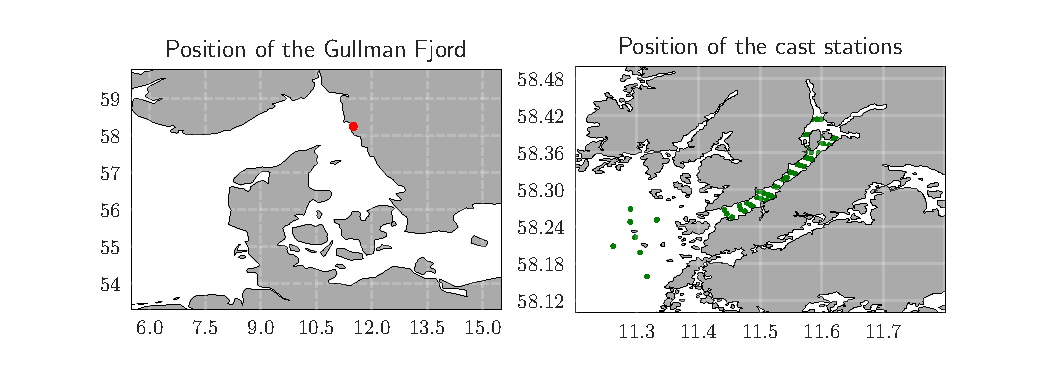
\includegraphics{stations}
  \caption{\label{fig:stations}Situation of the Gullmar Fjord (red dot) and position
    of the CTD casts (green dots).}
\end{figure}

Almost no work has been conducted during this study about
sub-mesoscale heat fluxes equivalent or about geostrophy,
mainly due to a lack of time.
The change of the field work because of the weather made me
focus on other physical processes.

\subsection{Data processing}
For a better readability, we will refer to potential temperature as temperature
and to absolute salinity as salinity.
If needed, we will explicitly use the term {\it in situ} to refer to
measured temperature and salinity.

To ensure coherence in the whole dataset and between the two ships,
all the data have been regridded on a 1 meter grid, from 0 to 119 meters depth.
Depths without any measurement points have been filled with NaN.

\paragraph{Conversion following TEOS-10}
Using the library provided by TEOS-10 \citep{gsw}, {\it in situ} temperatures and practical
salinities have been converted to potential temperature and absolute salinity.
Potential density anomaly has also been derived.

\paragraph{Calibration}
One cast has been conducted at the same position with the two ships each day,
so that all the measured variables can be calibrated between the two datasets.
The Skagerrak data have been chosen as reference data, because of a more
recent recalibration of the CTD sensors than the Trygve sensors.
After a linear regression between Trygve and Skagerrak calibration profiles
under the thermocline, the coefficients have been used to recalibrate
Trygve profiles for each day.
See Table~\ref{tab:calib} for the used coefficients.


\subsection{Turner angle}
One way to estimate the role of the salinity and the temperature on the stratification
is to use the Turner angle $Tu$ \citep{ruddick1983, johnson2012}:
\[Tu = atan2(\alpha \partial_z T + \beta \partial_z S,
\alpha \partial_z T - \beta \partial_z S),\]
with $\alpha$ the thermal expansion, $\beta$ the haline contraction,
$\partial_z T$ the vertical gradient of the temperature,
$\partial_z S$ the vertical gradient of the salinity,
and $atan2$ the four-quadrants inverse tangent.
If $Tu = 45\degree$ the temperature controls totaly the density changes,
if $Tu = -45\degree$ the salinity controls totaly the density changes,
at $0 \degree$ the temperature and the salinity control both equally
the density changes.
If $|Tu| > 45\degree$ the temperature and the salinity are working
one against the other, with total compensation if $|Tu| = 90$.
If  $|Tu| > 90$, the stratification is unstable, which is not the case in
our study.

The Turner angle has been computed at every depth for each profile,
using values of $\alpha$ and $\beta$ given by the TEOS-10 library.


%\subsection{Geostrophy TODO compute}
\subsection{Profile fitting and layers}
Temperature profiles in the fjord all look very similar, with
\begin{inparaenum}
\item an upper thermocline;
\item a warm water mass;
\item a lower thermocline;
\item the lowest layer where temperature is approximately constant.
\end{inparaenum}
It is not easy to compute the depth of these layer by using a threshold (on the
value or on the gradient) due to the irregularities of the temperature.
Inspired by the work of \cite{pauthenet2017}, we decided to approximate
the profiles with a function and then extract the layers information from the
functions properties. As the studied profiles have all the same shapes,
we used a mutli-linear fit, fitting the 4 layers.
The parameters of the fitted function are the depths and the temperatures
of the interface between each layers. We considered that for the lowest layer,
the fitted temperature will be a constant. An {\it a priori} model was set
for these 8 parameters, with values set by eye to be a good candidate.
Table~\ref{tab:apriori} in Appendix presents the parameters. The least squares
approximation has been used to find the best parameters.
For the profiles that are not deep enough, only the part where data are present
has been used for the least squares method. The {\it a priori} model
has been set for the lower part, with a confidence flag set to 0.
Figure~\ref{fig:fit} presents two examples of profiles: one where the 4 layers
are present and one where the fjord was not deep enough, so only
the upper layer is fitted.

\begin{figure}[h]
  \centering
  \includegraphics{{explainProfFit}}
  \caption{\label{fig:fit}Profile fitting with a multi-linear function.
    The measured profiles are plotted in green, the fitted functions in blue,
    and the red crosses represent depth and temperature at the interfaces
    between the different layers. On the right plot, the fit corresponds to the
    {\it a priori} model for the two lowest interfaces.}
\end{figure}

\section{Results}
%\paragraph{T and S profiles}
%\begin{figure}
%  \centering
%  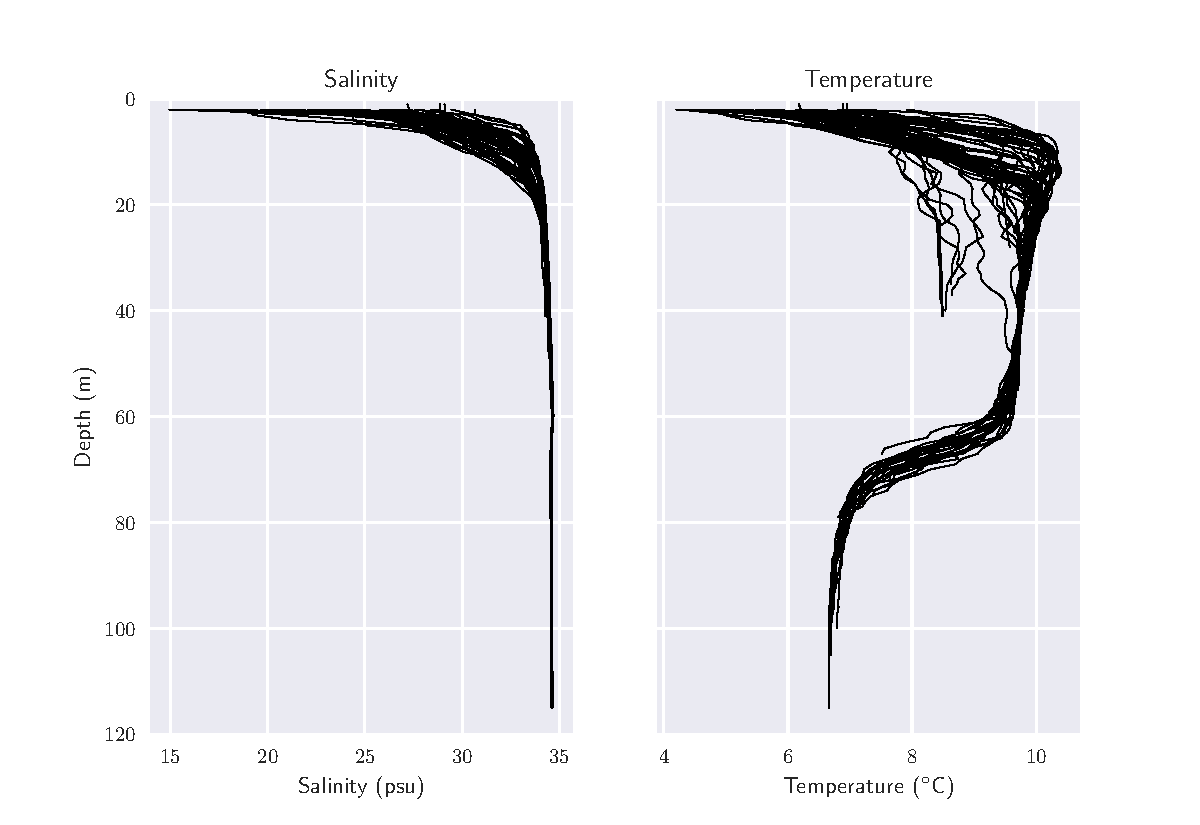
\includegraphics{profileTot}
%  \caption{\label{fig:proftot}Temperature and salinity profiles for all the casts.}
%\end{figure}

\begin{figure}
  \centering
  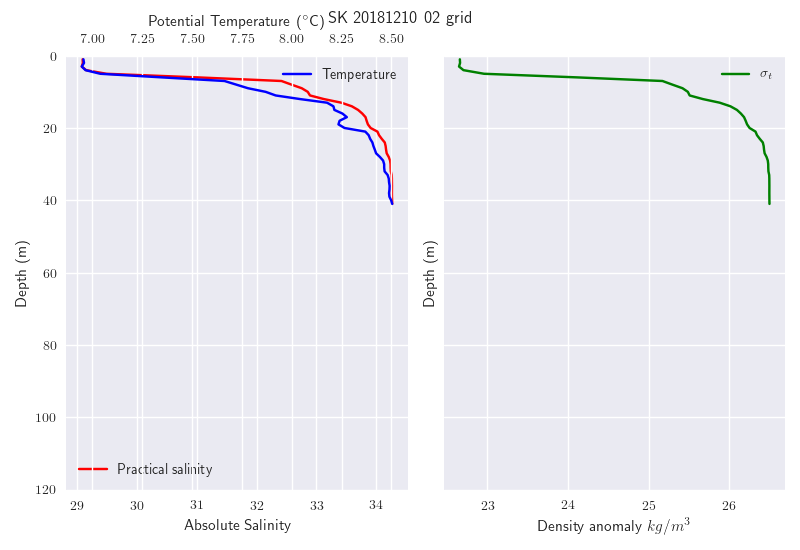
\includegraphics[width=\textwidth]{prof_offshore}
  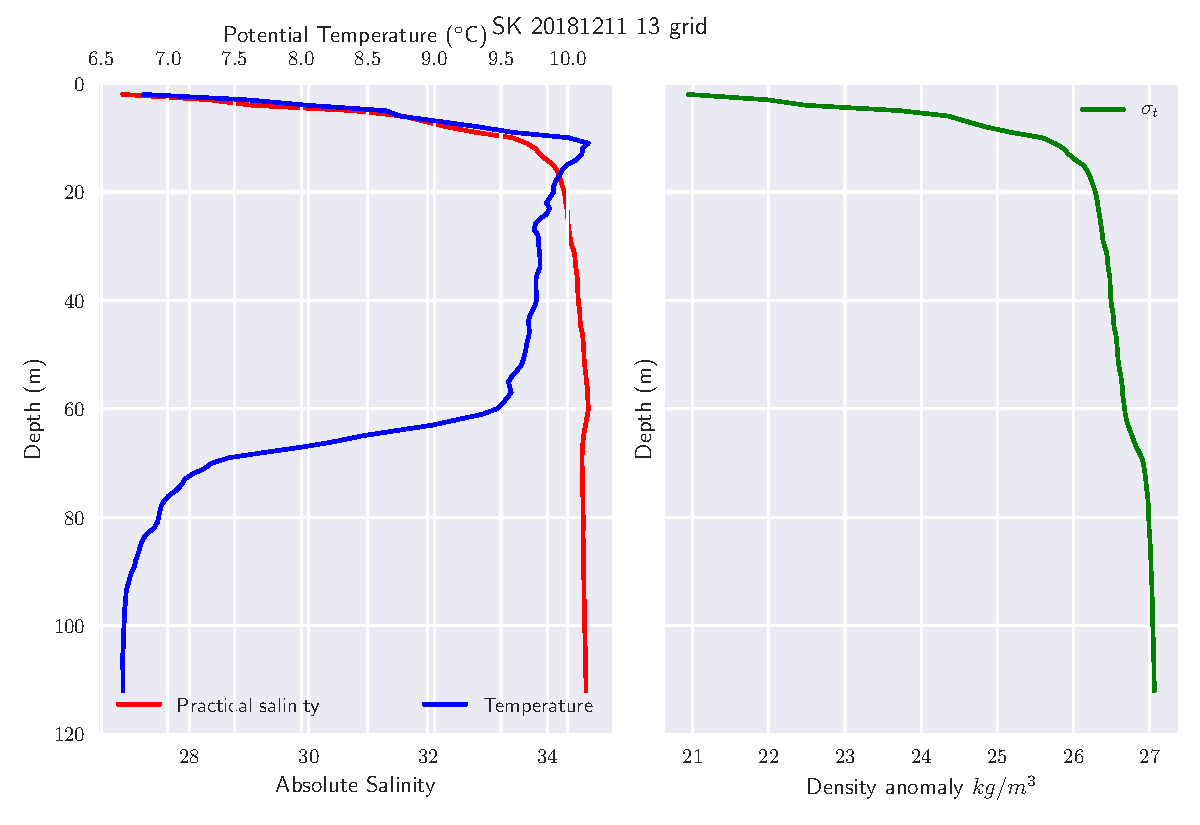
\includegraphics[width=\textwidth]{prof_fjord}
  \caption{\label{fig:profex}Example of two profiles, offshore on the top and in
    the Gullmar fjord on the bottom.
    These profiles are very representative of all the measured profiles.
    The emperature is in blue, the salinity is in red and the density anomaly
  is in green.}
\end{figure}
The offshore transect and the casts inside the fjord have different shapes
(Figure~\ref{fig:profex}).
A mixed layer of few meters is present offshore.
The salinity is around 29 at the surface of the offshore profile, increasing
along a sharp halocline to more than 34. The salinity is here representative
of Skagerrak water.
The temperature follows the same kind of shape: roughly constant
in the mixed layer and then increasing.
The density is increasing under the mixed layer, even if the temperature
increases, it is not sufficient to compensate the large variation
of the salinity, leading to a density controlled by the salinity here.

On the opposite, in the very calm
conditions of the fjord, no mixed layer is visible.
An upper layer of 10 to 20 meters controlled by a strong halocline
lies over a warm water mass, where density seems to follow the shape of
the salinity. The salinity changes a little bit in this warm water and in the lower layers,
but keeps values over 34 when the temperature variates from 10\,$\degree$C
to 9.5\,$\degree$C at the bottom of the warm water to reach a little
more than 6.5\,$\degree$C at the bottom.
Despite a slight decrease of the salinity after 60 meters, the density
seems to be controlled by the temperature variations of the lower thermocline.

%\paragraph{T-S diagram}
The 28 salinity limit in the fjord profiles is in the middle
of the upper cline. \cite{arneborg2003} presents an upper layer (around 10 meter
depth) of Kattegat water in the fjord during the summer, under which a halocline
and the Skagerrak water are present. The depth of the halocline is strongly related
to the inflow or outflow of water in the fjord.
Even if the Kattegat water seems to be present at the surface (Figure~\ref{fig:ts}),
the main part of the water is Skagerrak water. The upper cline
is visible on Figure~\ref{fig:ts}, as the mixing between the Kattegat (yellow points)
and the Skagerrak upper water (yellow/green points).
The salinity and the temperature of the bottom stagnant layer
have very little spatial variation.

\begin{figure}[h]
  \centering
  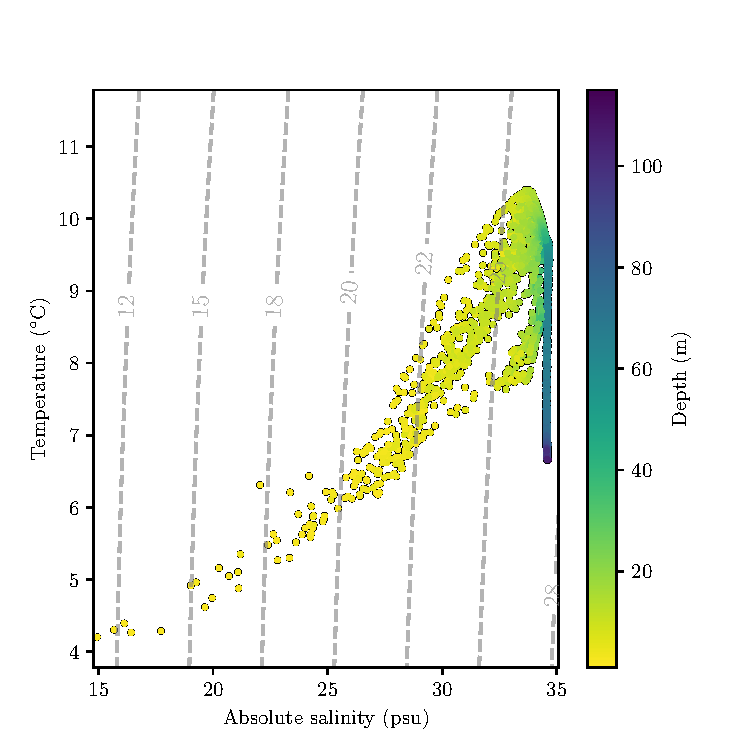
\includegraphics{ts}
  \caption{\label{fig:ts}T-S diagram regroupping all profiles. The color
    of points represents the depth.
    The dashed lines are the lines of constant density anomalies in kg/m$^3$.}
\end{figure}

%\paragraph{Turner angle}
\begin{figure}[h]
  \centering
  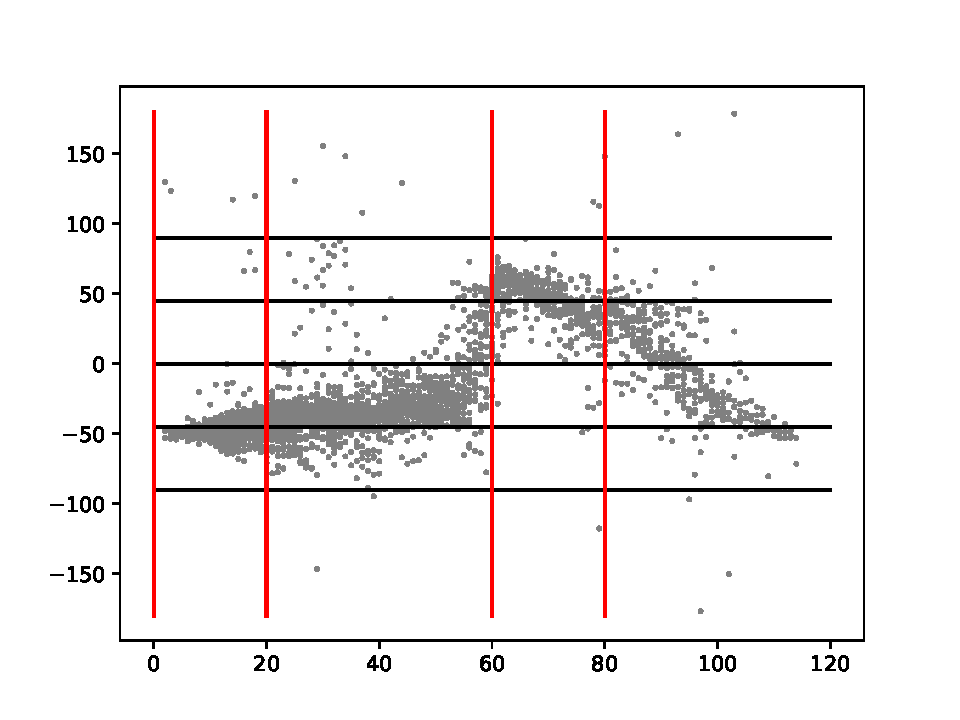
\includegraphics{turner}
  \caption{\label{fig:turner}Turner angle as a function of depth.
    Colors have been used to delimit the area where the temperature
    is the principal actor ($0<Tu<90$, green)
    and the area where the salinity controls the density changes ($-90<Tu<0$, blue).
    The red lines represent the mean position of the interfaces between the
    different water layers.}
\end{figure}
By a visual analyze, it has been seen that both the temperature and the salinity can control
the stratification, depending on the depth. This result is confirmed by the
Turner angle. To help the analyze, mean depth for each
fitted interface have been plotted in red in Figure~\ref{fig:turner}.
In the upper halocline, the Turner angle is indicating that the salinity
is almost totaly controlling the stratification, with a little opposite
effect of the temperature ($Tu_{mean} \simeq -48.5\degree$, $Tu_{std} \simeq 11.5\degree$).
This is consistant with the strong halocline that acts to densify the
water and the temperature augmentation that lightens the water.\\
On the second layer (warm water) the temperature decreases slightly,
while the salinity continues to increase.
$Tu$ is mainly situated between $-45\degree$ and $0\degree$
($Tu_{mean} \simeq -33.0\degree$,
$Tu_{std} \simeq 25.7\degree$), meaning that
the salinity and the temperature have the same effect on the stratification,
but the salinity still has the main impact.\\
The warm layer has a completely different behaviour:
$Tu_{mean} \simeq 48.4\degree$, $Tu_{std} \simeq 14.1\degree$.
The temperature is now the main actor of the stratification.\\
From 60 to 110\,m, the Turner angle decreases starting at an almost
only temperature controlled stratification to an almost only salinity controlled
stratification. This is due to the fact that the temperature decreases
on the lower thermocline but does not variate a lot at the bottom
of the stagnant water mass.\\
The stratification is mainly controlled by the salinity
and the the fjord would be classified as a Beta ocean
\citep{carmack2007}, but here this is the result of a strong halocline
which is a very different cause than the small sensibility of the density
to temperature at low temperature.

%\paragraph{Layers properties}
\begin{figure}[h]
  \centering
  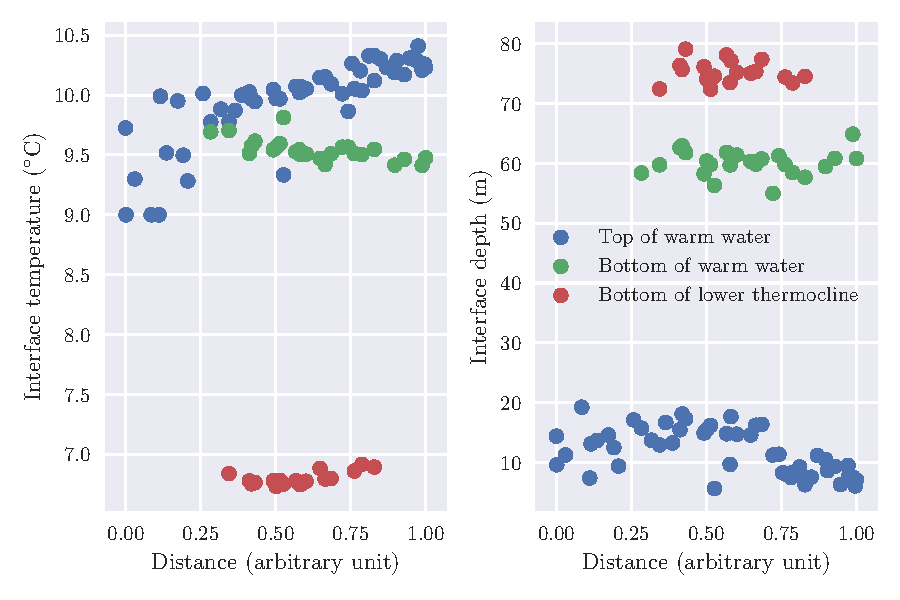
\includegraphics{layers}
  \caption{\label{fig:layers}Temperature and depth of the fitted interfaces
    between the water layer. The distance is expressed using an arbitrary unit,
    0 meaning near Kristineberg and 1 near the end of the fjord.}
\end{figure}
The interfaces between each water layers have been computed using
the temperature variations as described previously.
The temperature at the top of the warm water
increases from the beginning to the end of the fjord (Figure~\ref{fig:layers}) when
the temperature at the bottomn of the warm water
decreases slightly from the beginning to the end of the fjord.
The thickness of the warm water is minimum at the beginning of the fjord (42.6\,m),
maximum at the end of the fjord (57,3\,m), with a mean thickness of 47,6\,m
(standart deviation of 3.7\,m).
The spatial variations of the warm water boundaries depth can be
well seen on
Figure~\ref{fig:transect} and Figure~\ref{fig:layer_map}, on the Appendix.

\clearpage
\section{Discussion and conclusions}

Upwelling event are common in december \citep{bjork2003}, which agrees with
the wind direction present during the field work.
The top of the upper halocline is near to the surface,
signature of an upwelling and an inflow of Skagerrak warm water
in the fjord.
Despite this, the shape of the warm water would let imagine an outflow of
the warm water: the thickness is not coherent with an inflow
from the mouth of the fjord. This would need more attention,
particularly in term of internal waves and precise current velocities
to confirm or refute this remark.

The strong differences between the Skagerrak and the Kattegat water salinities
is at the origin of the salinity controlled density at the interface between
these two water types. The surface water (at least up to more than 30\,m)
temperature is following a seasonal cycle, from more than 15\,$\degree$C
at 5\,m during the summer to few degrees in the winter \citep{bjork2003}.
The strong thermocline is not sufficient to inverse the stratification
and then lead to a mixing of the two water masses.
The Turner angle only becomes positive under about 60\,m,
where the water is not subject anymore to the seasonal temperature cycle in
a non mixing environment.
The low salinity of the Baltic sea leads to a stratification controlled
by the temperature only at some depth where the temporal variations
of the temperature and the salinity are low.
This conduct to a three stable layered fjord: the Kattegat water lying
over Skagerrak water, and a stagnant mass is present at the bottom.
During the summer, the upper part of the water column is heated,
leading to a decreasing of the density of the surface layer, strengthening
the stratification.

% further work
The fitting of the profile with a mutli-linear funtion has been executed
for reasons of simplicity and leaded to good enough efficiency.
Using splines could give better fits, but the gain of accuracy could
be to the detriment of physical sense and the interfaces postion ease.
A mixed layer need to be added
if present on the data, but here also a linear fit has a physical sense, because
of homogeneity of the properties in the mixed layer.
The Turner angle can also be used to separate the different layers,
especially for the bottom of the warm water where the stratification becomes
governed by the temperature changes.
This would lead to better estimation of the thickness of the layers.
Associating the profile fitting with mooring data could also
be usefull to study internal waves.



%See what is the context
%Sk and Kat water, strong sal difference
The Gullmar fjord is situated in a coastal region where two main water
types are present: the salty Skagerrak water and the fresh Kattegat one,
that come from the Baltic sea.
%What we wanted to prove
%what is happening in term of water masses?
Skagerrak warm water comes inside the fjord, especially during upwelling events.
The average turnover time of these warm water is 40 days \citep{arneborg2003}.
%What we did
%a lot
The study of the processes that lead to a strong stratification as well as
the analyze of the layer properties has been conducted with data acquired
durinf a two-days field campaign.
%What we showed/saw
%stable
The main result is that the stratification is very stable, mainly leaded
by the salinity, not because a cold temperature but because of
very high salinity variations.
%What is the conclusion
%-> stable, shape will not change
The temperature variations induced by the seasonal cycle are not strong
enough to counterbalance the halocline. The shape of the profiles,
coming from the intrinsic properties of the Baltic sea and the Atlantic
ocean are not suspect to major changes, except for interfaces depth variations.

\clearpage
\newpage

\bibliographystyle{../Biblio/agufull08}
\bibliography{../Biblio/biblio}

\newpage

%\renewcommand\thefigure{\thesection.\arabic{figure}}
\appendix

\section{Appendix}

\begin{table}[h]
  \centering
  \begin{tabular}{|l|c|r|}
    \hline
    Depth (m) & Temperature ($\degree$C) & Comment \\
    \hline
    0 & 5 & Surface\\
    20 & 10 & Bottom of the upper thermocline / top of the warm water\\
    60 & 9 & Bottom of the warm water / top of the lower thermocline\\
    80 & 7 & Bottom of the lower thermocline / top of the lowest layer\\
    \hline
  \end{tabular}
  \caption{\label{tab:apriori}Values of the {\it a priori} model for the multi-linear fit.}
\end{table}

\begin{table}[h]
  \centering
  Temperature\\
  \begin{tabular}{|l|c|c|}
    \hline
    Date & $a_T$ & $b_T$ \\
    \hline
    2018-12-10 & 0.9938598212928323461 & 0.07856246515108189499\\
    2018-12-11 & 1.006636216123387273  & -0.09514920786826941423\\
    \hline
  \end{tabular}
  
  \vspace{.5cm}
  Salinity\\
  \begin{tabular}{|l|c|c|}
    \hline
    Date & $a_S$ & $a_S$ \\
    \hline
    2018-12-10 & 0.8453445700814513630 & 5.276859099581269419\\
    2018-12-11 & 0.8190729895351881451 & 6.231978296168669829\\
    \hline
  \end{tabular}
  \caption{\label{tab:calib}Regression coefficients, the calibration has the following
    shape:
    ${X_{Trygve} = a_X \cdot X_{Skagerrak} + b_X}$, with $X$
    the temperature or the salinity.}
\end{table}

\begin{figure}
  \centering
  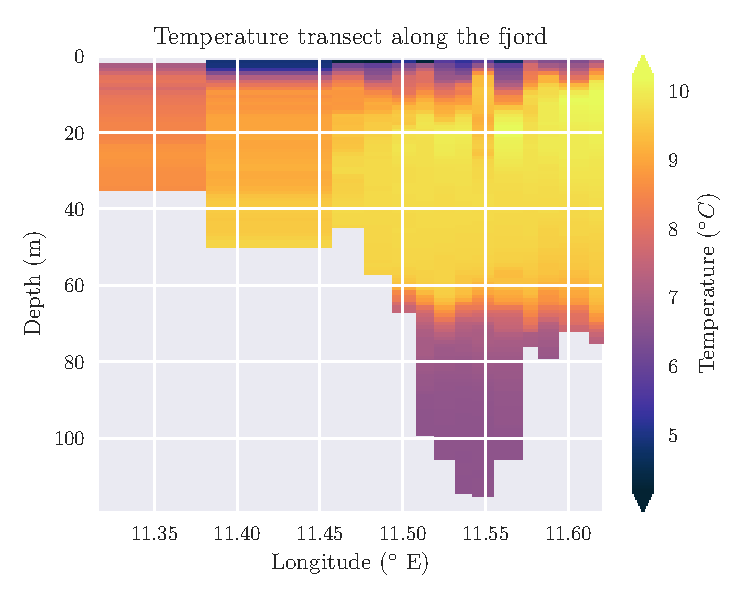
\includegraphics{transect}\\
  \caption{\label{fig:transect}Transect of the temperature along the fjord.
    The top of the warm water is deeper at the beginning of the fjord than
    at the end. On the contrary, the bottom of the warm water is deeper at the
    end of the fjord, leading to a thinner warm layer at the beginning
  of the fjord.}
\end{figure}
\begin{figure}
  \centering
  \includegraphics{{layer_bottom_of_thermocline}}
  \includegraphics{{layer_bottom_of_warm_water}}
  \caption{\label{fig:layer_map}Map of the depth of the top and the bottom of the warm water.}
  
\end{figure}
\end{document}
